% This is "sig-alternate.tex" V2.0 May 2012
% This file should be compiled with V2.5 of "sig-alternate.cls" May 2012
%
% This example file demonstrates the use of the 'sig-alternate.cls'
% V2.5 LaTeX2e document class file. It is for those submitting
% articles to ACM Conference Proceedings WHO DO NOT WISH TO
% STRICTLY ADHERE TO THE SIGS (PUBS-BOARD-ENDORSED) STYLE.
% The 'sig-alternate.cls' file will produce a similar-looking,
% albeit, 'tighter' paper resulting in, invariably, fewer pages.
%
% ----------------------------------------------------------------------------------------------------------------
% This .tex file (and associated .cls V2.5) produces:
%       1) The Permission Statement
%       2) The Conference (location) Info information
%       3) The Copyright Line with ACM data
%       4) NO page numbers
%
% as against the acm_proc_article-sp.cls file which
% DOES NOT produce 1) thru' 3) above.
%
% Using 'sig-alternate.cls' you have control, however, from within
% the source .tex file, over both the CopyrightYear
% (defaulted to 200X) and the ACM Copyright Data
% (defaulted to X-XXXXX-XX-X/XX/XX).
% e.g.
% \CopyrightYear{2007} will cause 2007 to appear in the copyright line.
% \crdata{0-12345-67-8/90/12} will cause 0-12345-67-8/90/12 to appear in the copyright line.
%
% ---------------------------------------------------------------------------------------------------------------
% This .tex source is an example which *does* use
% the .bib file (from which the .bbl file % is produced).
% REMEMBER HOWEVER: After having produced the .bbl file,
% and prior to final submission, you *NEED* to 'insert'
% your .bbl file into your source .tex file so as to provide
% ONE 'self-contained' source file.
%
% ================= IF YOU HAVE QUESTIONS =======================
% Questions regarding the SIGS styles, SIGS policies and
% procedures, Conferences etc. should be sent to
% Adrienne Griscti (griscti@acm.org)
%
% Technical questions _only_ to
% Gerald Murray (murray@hq.acm.org)
% ===============================================================
%
% For tracking purposes - this is V2.0 - May 2012

\documentclass{sig-alternate}

\begin{document}
%
% --- Author Metadata here ---
\conferenceinfo{WSDM}{'2016 San Francisco, USA}
%\CopyrightYear{2007} % Allows default copyright year (20XX) to be over-ridden - IF NEED BE.
%\crdata{0-12345-67-8/90/01}  % Allows default copyright data (0-89791-88-6/97/05) to be over-ridden - IF NEED BE.
% --- End of Author Metadata ---

\title{Question Answering using Structured and Semi-structured User Generated Content}
%
% You need the command \numberofauthors to handle the 'placement
% and alignment' of the authors beneath the title.
%
% For aesthetic reasons, we recommend 'three authors at a time'
% i.e. three 'name/affiliation blocks' be placed beneath the title.
%
% NOTE: You are NOT restricted in how many 'rows' of
% "name/affiliations" may appear. We just ask that you restrict
% the number of 'columns' to three.
%
% Because of the available 'opening page real-estate'
% we ask you to refrain from putting more than six authors
% (two rows with three columns) beneath the article title.
% More than six makes the first-page appear very cluttered indeed.
%
% Use the \alignauthor commands to handle the names
% and affiliations for an 'aesthetic maximum' of six authors.
% Add names, affiliations, addresses for
% the seventh etc. author(s) as the argument for the
% \additionalauthors command.
% These 'additional authors' will be output/set for you
% without further effort on your part as the last section in
% the body of your article BEFORE References or any Appendices.

\numberofauthors{1} %  in this sample file, there are a *total*
% of EIGHT authors. SIX appear on the 'first-page' (for formatting
% reasons) and the remaining two appear in the \additionalauthors section.
%
\author{
% 1st. author
\alignauthor
Denis Savenkov\\
       \affaddr{Emory University}\\
       \affaddr{Atlanta, USA}\\
       \email{denis.savenkov@emory.edu}
}

\maketitle
\begin{abstract}
Modern question answering (QA) systems employ a variety of different unstructured (text corpora), semi-structured (question answer pairs, infoboxes) and structured (knowledge bases) data sources for candidate generation.
However, typically each of the data sources is processed independently and the merging of the results happen only after the candidates are generated.
I propose to enrich the expressiveness of data representation of each of the data sources with complimentary information for joint reasoning.
More specifically, text documents that mention entities from a knowledge base (KB) can be extended with the information about properties and connections of these entities, and text fragments mentioning the entities and relations can help knowledge base question answering systems to find a good mapping between natural language questions and the corresponding structured query representations.

% This is probably not that related.
% I also propose to use existing QnA pairs from community question answering (CQA) websites both as training data for both text- and KB-based question answering systems.

\end{abstract}

% A category with the (minimum) three required fields
\category{H.3.3}{H.3.3 Information Search and Retrieval}{Retrieval models}
\category{I.2.3}{Artificial Intelligence}{Answer/reason extraction}

\keywords{Question Answering; Knowledge Bases; Web Search}

\section{Introduction}
Traditionally question answering systems used text document collections to retrieve passages relevant to a question and to extract candidate answers \cite{Vrandecic:2014:WFC:2661061.2629489}.
Unfortunately, a paragraph of text encodes a very limited amount of information about answer candidates and predictions has to be used instead, \eg most of the systems estimate candidate answer entity type to match against the expected type inferred from the question text.
On the other hand, modern large scale open-domain knowledge bases, such as dbPedia \cite{auer2007dbpedia}, Freebase \cite{Bollacker:2008:FCC:1376616.1376746} and WikiData \cite{Vrandecic:2014:WFC:2661061.2629489} store a vast amount of general knowledge about different kinds of entities.
This information, encoded as \texttt{[subject, predicate, object]} RDF triples, can be effectively queried using structured query languages, such as SPARQL.
Of course, regular users would rather prefer to ask natural language questions.
Translation of text questions into structured query languages is very challenging for a number of reasons: complexity of a KB schema, variability of natural language and knowledge representation \etc
For example, Figure \ref{fig:example_sparql} gives a SPARQL query that retrieves the answer to a relatively easy question \textit{``who is the current president of the dominican republic in 2010?''}.
% The same information can be asked in many different ways, for example: \textit{``who is the dominican republic president in 2010?''}, or \textit{``who was the leader of the dominican republic in 2010?''} \etc

\begin{figure*}
\centering
\begin{lstlisting}[frame=single]
PREFIX : <http://rdf.freebase.com/ns/>
SELECT DISTINCT ?name {
   :m.027rn :government.governmental_jurisdiction.governing_officials ?gov_position .
   ?gov_position :government.government_position_held.basic_title :m.060c4 .
   ?gov_position :government.government_position_held.office_holder ?president .
   ?gov_position :government.government_position_held.from ?from_date .
   ?gov_position :government.government_position_held.to ?to_date .
   FILTER (
       xsd:date(?from_date) <= "2010"^^xsd:date AND
       xsd:date(?to_date) >= "2010"^^xsd:date
   )
   ?president :type.object.name ?name
}
\end{lstlisting}
\caption{SPARQL query that retrieves the answer to the query \textit{``who is the current president of the dominican republic in 2010?''}}
\label{fig:example_sparql}
\end{figure*}

\begin{figure}
\centering
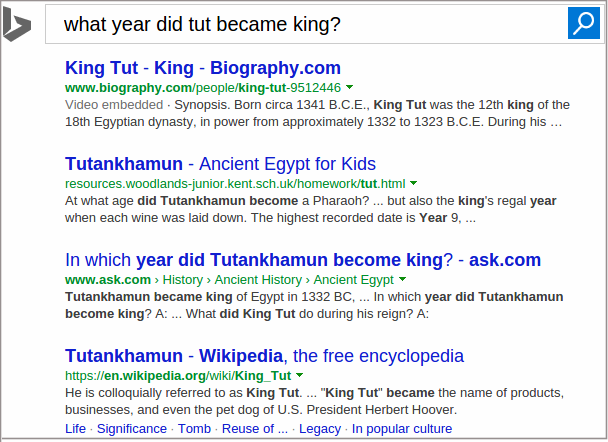
\includegraphics[width=0.5\textwidth]{img/web_search_entitylink}
\caption{Search results for the question ``what year did tut became king?''}
\label{fig:web_search_entitylink}
\end{figure}

The first problem that a KBQA system is facing is question entity identification.
The performance of the whole system greatly depends on this stage \cite{yao-scratch-qa-naacl2015}, because it seeds the answer candidate search process.
Question text is often quite short, may contain typos and other problems, that complicate question entity identification.
Existing approaches are usually based on dictionaries that contain entity names, aliases and some other phrases, which were used to refer to entities \cite{SPITKOVSKY12.266}.
These dictionaries are often noisy and incomplete, \eg to answer the question \textit{``what year did tut became king?''} a system needs to detect a mention \textit{``tut''}, which refers to the entity \textit{``Tutankhamun''}.
A mapping \textit{tut $\rightarrow$ ``Tutankhamun''} is missing in the dictionary used by one of the state of the art systems and therefore it couldn't answer this question correctly.
Instead of increasing the dictionary size we propose to use web search results to find variations of question entity names, which can be easier to link to a KB.
This idea was used for entity linking in web search queries \cite{SMAPH_ERD:2014}, which was given as one of the tracks on the Entity Recognition and Disambiguation Challenge 2014\footnote{http://web-ngram.research.microsoft.com/ERD2014/}.
Figure \ref{fig:web_search_entitylink} presents web search results for the query \textit{``what year did tut became king?''}, which shows that indeed many documents mention the full name, which can easily be mapped to a KB entity.

After question entities have been identified the next step is to explore their neighborhood and build structured queries as candidate answers.
A query addresses one or multiple KB predicates, which should be somehow related to words and phrases in the question and systems try score these mappings in order to select the best answer.
Existing knowledge base question answering approaches \cite{ACCU:2015,Berant:EMNLP13,berant2014semantic,berant2015imitation,BordesCW14:emnlp,yao2014freebase} rely on some kind of a lexicon, which is learned from manually labeled training data and supported by some additional resources, such as question paraphrases \cite{berant2014semantic} and weakly labeled sentences from a large text collection \cite{yao2014information}.
However, given the fact that manually labeled training data is very limited, such lexicons do not cover thousands of different predicates present in a KB.
By our estimate in a popular WebQuestions KBQA dataset answers to $\sim$5.5\% of test questions (112 out of 2032) involve a predicate, that doesn't appear in the training set.
For example, an RDF triple \texttt{[Bigos, food.dish.type\_of\_dish1, Stew]} answers a test question \textit{``what are bigos?''}, but there are no questions from the training set that are answered using the same predicate.
In addition, even if training set contains an example targeting a particular KB predicate, the lexicon might not cover all the other possible ways the same information can be asked about.
For example, test question \textit{``who is the woman that john edwards had an affair with?''} is similar in meaning and is answered with a similar query as a training set question \textit{``who did jon gosselin cheat with?''}, but the word \textit{affair} isn't used in the training set.
On the other hand, traditional text-based question answering systems benefit from the redundancy with which the same information is stated in many different ways in many documents \cite{Lin:2007:EPU:1229179.1229180}.
This increases the chances of a good lexical match between a question and answer statements, which makes even some relatively simple counting-based techniques quite effective \cite{brill2002analysis}.
We propose to borrow some ideas from text-based question answering and enrich the representation of candidate structured queries with additional text documents and fragments, that can help to select the best answer.
For example, the right part of the Figure \ref{fig:model} shows web search results, community question answering page and text fragments mentioning pairs of entities, that can clearly be useful to answer the question about John Edwards' affair.

\subsection{Contributions}

Our main contributions in this work are three-fold:
\begin{itemize}
\item a novel ``hybrid'' knowledge base question answering system, which uses both structured data from a knowledge base and unstructured natural language resources connected via entity links. Section \ref{section:method} describes the architecture of our system, and Section \ref{section:eval} shows that this fusion improves the performance of a state of the art KBQA system.
\item novel data sources for knowledge base question answering. Entity linking allows us to connect test resources with a KB. We explore three different types of text data, that is useful for KBQA: web search results (Section \ref{section:method:web}), Community Question Answering data (Section \ref{section:method:cqa}) and entity pairs language model based on a large text corpus (Section \ref{section:method:clueweb}).
\item evaluation and analysis. We evaluate the performance of our system on a popular WebQuestions dataset and demonstrate that using additional text resources we can improve the quality of knowledge base question answering (Section \ref{section:eval}). In addition, we conduct an extensive analysis of the system and suggest directions for future research (Section \ref{section:analysis}).
\end{itemize}

% -------------------------------------------

%There are many problems in KBQA:
%\begin{itemize}
%\item lexical variations, we can call the same thing in million ways
%\item representation variation - similar data can be represented in multiple ways, e.g. capital of the state in Australia location.australian\_state.capital\_city, while in the US you will have totally different predicate. HOWEVER, these are old predicate and marked deprecated. There is another predicate that should be the same for both cases.
%\item Incomplete, some data is simply missing or details are not present. E.g. who is the woman that john edwards had an affair with?, there is a triple that says that he had sexual relationships with Rielle Hunter, but there is no details...
%\item Related to the previous - many predicates are simply not present. There is something related, but not exactly what is asked about. Example: where did andy murray started playing tennis? We can find the answer entity, but the triple won't say that he started playing there.
%\end{itemize}

%In \cite{Sun:2015:ODQ:2736277.2741651} authors report pretty low score for Sempre on TREC and Bing QA datasets.

% Questions and corresponding answers are often expressed differently and researchers in question answering studied different ways to bridge this lexical gap, \eg using translation models \cite{Murdock:2005:TMS:1220575.1220661} and distributional semantics \cite{yu2014deep}.




\section{Related Work}
\input{related_work.inc}

\section{Research Proposal}
\input{proposal.inc}

\section{Experiments}
\input{experiments.inc}

\section{Discussion}
\input{issues.inc}

%
% The following two commands are all you need in the
% initial runs of your .tex file to
% produce the bibliography for the citations in your paper.
\bibliographystyle{abbrv}
\bibliography{sigproc}  % sigproc.bib is the name of the Bibliography in this case
% You must have a proper ".bib" file
%  and remember to run:
% latex bibtex latex latex
% to resolve all references
%
% ACM needs 'a single self-contained file'!
%
%APPENDICES are optional
%\balancecolumns
\appendix
%Appendix A
\section{Why I want to attend the doctoral consortium}
During the course of my studies I've worked on a number of different topics, starting from click log analysis, mobile user behavior analysis, search user assistance and recently I've pivoted to information extraction and question answering.
Having focused on a general direction of my future research I would definitely benefit from attending the WSDM Doctoral Consortium, which would let me get an extended feedback from experienced researchers with potentially different views of the problem.
The topic of the proposed research involves several related areas, namely information retrieval, natural language processing, web search and mining, knowledge representation and knowledge base construction and querying.
Therefore, I would greatly appreciate a chance to discuss the proposed direction with researchers with experience in these areas.
This would complement the experience of my advisor and hopefully make my thesis work more useful for the community.

\section{A paragraph from the advisor}
A brief statement (1 paragraph) by their advisor saying how the student would benefit by attending the Consortium. Advisors should also specifically state whether the student has written, or is close to completing, a thesis proposal (or equivalent), and when they expect the student would defend their dissertation if they progress at a typical rate.

\end{document}
